%************************************************
\chapter{Automatic programming}\label{ch:code-gen}
%************************************************

\begin{flushright}{\slshape Writing machine code involved several tedious steps—breaking down a process into discrete instructions, assigning specific memory locations to all the commands, and managing the I/O buffers. [...] We needed to understand how we might reuse tested code and have the machine help in programming. [...] This led to the development of interpreters, assemblers, compilers, and generators—programs designed to operate on or produce other programs, that is, automatic programming.} \\ \medskip
    --- Mildred ``Milly'' Kross
\end{flushright}

Creating a computer program is a challenging and engaging experience, it requires expertise, brilliance and ingenuity. At the same time, writing code is a mundane and dull activity, it requires to complete repetitive tasks, to manage multiple small issues and to deal with problems unrelated with the main project.

Thankfully, today, we are not dealing with the same difficulties that Mildred Kross faced when working on the UNIVAC I. Multiple technological advancements and progresses in Computer Science gave us compilers, high-level programming languages, design paradigms, frameworks, middleware, integrated development environments, and more. All these tools exist to make computer programming more about designing and developing a program than writing code. 

During Computer Science history, the concept of automatic programming changed to adapt to the expectation of the time. Originally, it was the automation of the process of punching paper tape, later it became the transformation of high-level programming languages (\eg, Fortran and ALGOL) to machine code, a task that, nowadays, is integral part of the build process. Today, automatic programming mostly refers to the automatic generation of executable code from representations that are not programming languages. These representation may have different level of abstraction, from the closest to the target (\eg, domain specific languages, flowcharts, \etc) to the furthest (\eg, graphical representations, models, \etc).

Here we present our approach to automatically generate a ROS architecture from an AADL model combined with a data description model. The chapter starts with a description of our target, specifically, an engineered version of a ROS nodes including advanced functionalities. Then the automatic programming process is presented with its two-steps approach. The chapter closes with an example going from model to code.

\minitoc
\newpage

\begin{figure}[t]
    \centering
    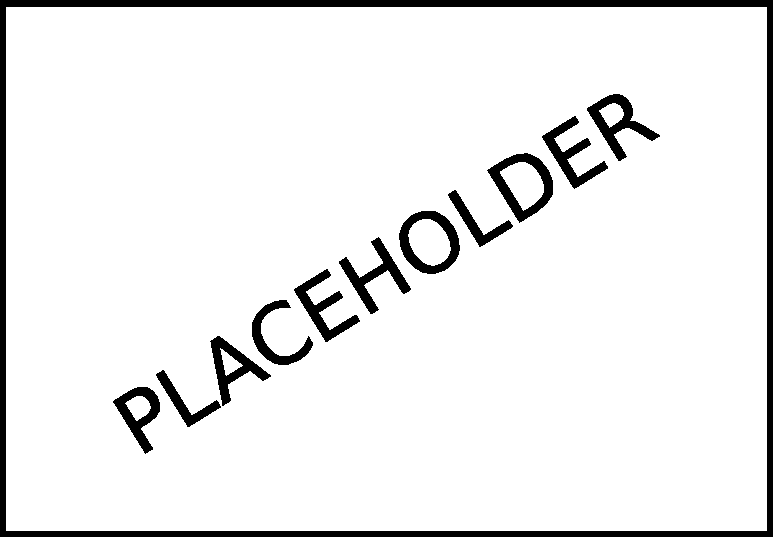
\includegraphics[width=0.8\textwidth]{gfx/placeholder}
    \caption{TODO}\label{fig:code-gen}
\end{figure}

\section{Generating ROS artefacts}
An automatic programming approach is a collection of rules and methods to transform an initial description to a different, more complex output. Therefore, even before the definition of the transformation itself it is necessary to define the input and the output of the process. In Chapter~\ref{ch:Modelling} we described in details a collection of meta-models that can be used to define ROS architectures using AADL in combination with a data modelling language (\ie, ANS.1 or JSON schema). A model compatible with this meta-models is the starting point of our automatic code generation process. Since the expected output of the entire process is a complete working architecture, the model alone is not enough as an input. To have a functioning architecture, the designer needs to pair the model definition with the implementation of the node inner functionalities; this can be done by using AADL properties. A ROS complete architecture is composed by multiple elements: existing nodes run as external resources, new nodes and messages created by the developers, launch files to organize the architecture, parameter profiles to configure the system. All these elements are  captured by the model, and can be automatically generated by our process. First, the automatic programming system creates the source code for the new custom nodes, the target language is C++. ROS supports multiple languages, mainly C++ and Python, Lisp is officially in the list but rarely used, and there are experimental libraries for Java and Lua. From the ROSwiki, \textit{rospy} (\ie, the Python implementation of ROS) is suggested as the approach that promotes implementation speed (\ie, reduced development time) over runtime performance, and it is designed specifically for fast prototyping, testing and lightweight implementations (\eg, configurations and initialisations), while \textit{roscpp} (\ie, the C++ implementation of ROS) is considered the main library, and it is designed with a focus on high performances and runtime speed. Since the output of the automatic programming is at the end of a long process involving a model-based design and carefully development components, we decided to use \textit{roscpp}, and therefore C++, as the target library to achieve the most efficient and robust implementation. Since C++ is a compiled language, the system will automatically generate all the necessary files to build the node executables; if the designer specify all the necessary information in the model (\ie, source code of the functionalities), the final output of the automatic programming process will be ready to compile with no intervention required. The automatically generated code will be placed in the correct package structure expected by ROS, together with any custom message, service or action file. This covers everything necessary for the execution of single nodes, to put them together in an architecture it is necessary to create launch files. In launch files, the designer specifies the instances of the nodes and how they are connected, by renaming all the necessary topics, and configured, by including configuration files. The topology of the architecture can be automatically extracted from the model and converted in a launch files, and the parametrisation defined using a data modelling language (\ie, ANS.1 or JSON schema) can be converted in the YAML description used by ROS. Moreover, in launch files existing nodes are included in the architecture and connected to the rest of the topology.

Figure~\ref{fig:code-gen} summarises the complete process. Our automatic programming approach requires as input a model defined in AADL, completed by a data description using ASN.1 or JSON schema, and specialised via properties to include functionality-specific source code. When all these conditions are met, the process provides as an output a collection of automatically generated and compilation-ready ROS nodes, their associated communication files (\ie, messages, service and action files) and the necessary launch files to run the architecture. A fully complete model creates an architecture that only needs to be compiled and run.

\begin{figure}[t]
    \centering
    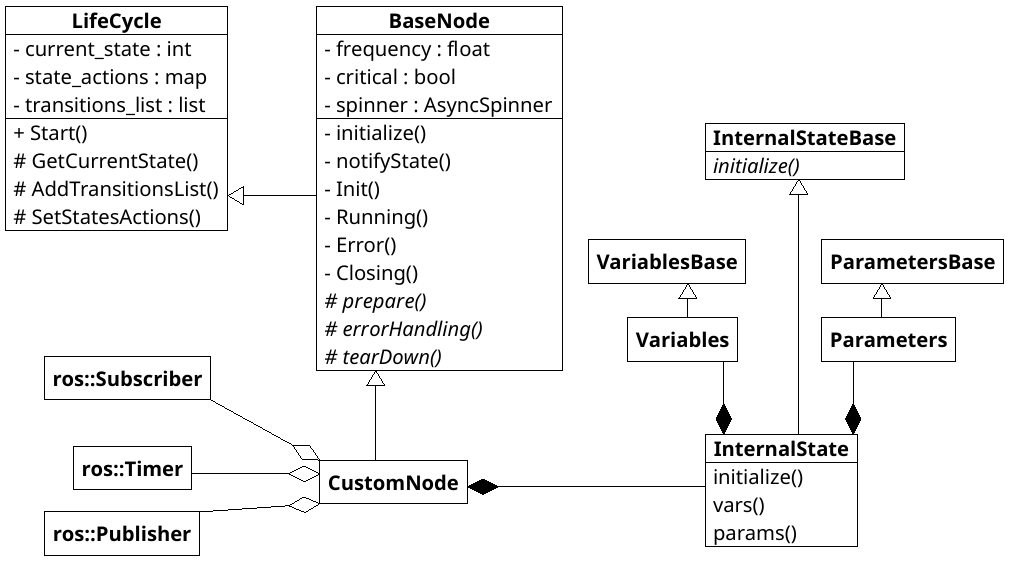
\includegraphics[width=\textwidth]{gfx/class}
    \caption{TODO}\label{fig:node-class}
\end{figure}

\section{Engineered ROS node}
\label{sec:ros-node}
Differently from other middleware or frameworks, ROS does not constrain the developer on the structure of the components; it was designed to be maximally flexible following the mantra: ``\textit{we don't wrap your main()}''. While this approach certainly contributed to the popularity and growth of ROS as a middleware and de facto standard for robotics, at the same time it created a very heterogeneous landscape for ROS nodes. Some of them are well designed, rich in functionalities, robust and configurable, others are cobbled together for a prototype and then used as legacy code for one single core functionality. Often this second category is created by experts in a specific field (\eg, vision, control, manipulation, \etc) that lack the necessary programming and software engineering skills and knowledge to develop a well-designed and robust node. With our approach we are targeting specifically this category of developers, that posses the expertise to contribute to the robotic community, but are discouraged by the programming required.

Since ROS does not impose any structure for the node, the simplest approach for automatic code generation would be to target an essential node, covering the minimum functionalities required to run it. There are few advantages in this approach: easier to implement code generator, simpler and more readable output, an implementation closer to what the developer knows. However, such a direct approach would have significant downsides: a lax relationship between the node and its model, lack of advanced functionalities that can be hidden in the automatic programming approach, less flexibility of the implemented node, more work left to the developer (\eg, testing, debugging, performance evaluation, \etc), more tampering by the developer with the basic structure of the node, no real benefit between a handcrafted and an automatically generated node. For all these reasons we decided to created an engineered base node that can be used as a reference and starting point for automatic code generation.

%TODO may not be simplified in the final version
Figure~\ref{fig:node-class} shows a simplified UML diagram of a custom node based on the engineered ROS node. Immediately, it is possible to recognise three main components: \textit{LifeCycle}, \textit{ROSNode}, and \textit{InternalState}. Each of them represent one of the main characteristics captured by the engineered node. The \textit{LifeCycle} implements an internal state machine that controls the evolution of the node. The \textit{ROSNode} is the core implementation of the node, capture all the ROS-related functionalities and management procedures. The \textit{InternalState} capture all the developer-defined parameters and variables necessary for the correct execution of the node.

\subsection{Life cycle}
When working with component-based approaches, it is important to define a recurring and consistent behaviour of the component, in the case of robotic components it is even more important, since they often operate with strict timing constraints and implement critical functionalities. In Section~\ref{sec:ros-in-aadl}, we presented how a life cycle of a node can be modelled in AADL, and how it can be used to guide the initialisation, configuration and execution of a component. To capture the same behaviour in the engineered node, we developed the \textit{LifeCycle} class to define the evolution of the node. While various implementations of state machines in C++ already exists, a very popular one has been around for almost 20 years\footnote{https://www.codeproject.com/Articles/1087619/State-Machine-Design-in-Cplusplus-2}, we opted to create a stripped down version that trades some functionalities for simplicity, understandability, and modern development approaches. The result is a very lightweight state machine, that supports dynamically defined states and transitions and it is completely ROS-independent.

To maintain the generality of the implementation, the class itself does not specify any state or transition. It only defines an empty enumeration that the subsequent classes can extend to define their own states. The valid transitions are defined as a list of pairs, going from one state to another, as for the states, the list is created by classes extending or using the state machine. The last initialisation step before running the state machine is to bind each state to a function. In practice, the binding is done by creating a map with the state as the key and a \texttt{std::fuction} as the value. Class template \texttt{std::function} is a general-purpose polymorphic function wrapper, it can be assigned to any callable target (\eg, functions, lambda expressions, pointers to member functions, \etc), this makes this approach particularly flexible and not bound to any specific implementation. When the initialisation is complete, the state machine can be started, the initial state is the one defined in the constructor, but there is no specific definition for a termination state. At each execution loop, first, the state machine execute the function bound to the specific state, then, it checks if there is a valid transition waiting to be performed, if there is one, the loop repeats and a new state-bound function is executed, otherwise the state machine has reached a final state and the execution terminates. While the list of all possible transitions is defined during the initialisation phase, each specific change of state is defined at runtime in all the state-bound functions. This is necessary, for example, to distinguish between a successful component initialisation that goes from an initial to a running state, to an unsuccessful one that would take the component to an error state. In practise, at the end of each state-bound function, the developer needs to specify the next state depending on the current outcome of the execution, then the state machine will check if the transition is valid (\ie, it is in the transitions list) and execute it. Mirroring the model presented in Section~\ref{sec:ros-in-aadl}, the engineered node supports five different states: initialisation, running, error report and closing. How they are implemented, what is their role and which ROS functionalities they evoke will be detailed in the next section.

\begin{figure}[t]
    \centering
    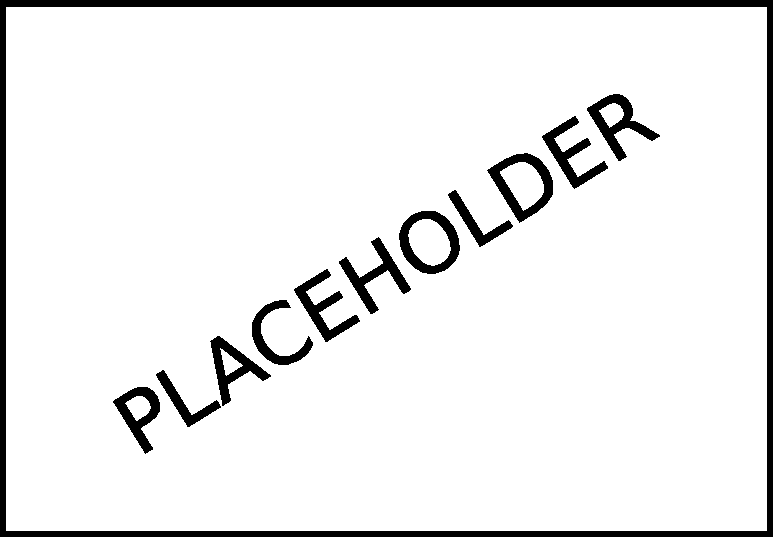
\includegraphics[width=0.8\textwidth]{gfx/placeholder}
    \caption{TODO}\label{fig:state-machine}
\end{figure}

\subsection{ROS node}
The core implementation of the engineered ROS node is in the \textit{ROSNode} class, here the life cycle is defined and materialised, and all the basic ROS-related functionalities are implemented. By defining this class, we can streamline the development process of a component by hiding the base initialisation procedure of a ROS node, create a well defined structure the developer can follow, and enhance the base implementation by adding additional functionalities (\eg, error detection and state report). The \textit{ROSNode} class extends directly the \textit{LifeCycle} class, therefore, the first implementation step is to define the states, the valid transitions and method bound to each state. Figure~\ref{fig:state-machine} presents the complete definition of the internal state machine, this mirrors the description provided in Section~\ref{sec:ros-in-aadl}. Each state is bound to a specific method of the class, and it implements a core functionality of the node.

\paragraph{Init} This method is bound to the initial state of the node (\ie, \texttt{ST\_INIT}). It is defined as a two-steps process and all the initialisation procedures of the component are implemented here.

The first step is a common initialisation that applies to every node, it sets up the ROS environment and defines the asynchronous spinner\footnote{http://wiki.ros.org/roscpp/Overview/Callbacks and Spinning}. In Section~\ref{sec:ros-in-aadl}, we modelled the ROS node with a external port to communicate the current state of the node after every transition, in this phase of the initialisation, the base node create the connection with the ROS service in charge of receiving this notifications. In ROS, a client can register to a service even if the server is not active, all the communications are lost until the service is finally started. This behaviour is not a problem for a status notification system, since it is meant to exist only to supervise the general evolution of the internal life cycle of the node. Nevertheless, our aim is to create a flexible base node that can adapt to different situations, thus, we defined an extra configuration property for the node, the developer can initialise the node as \textit{critical}. When a node is critical, instead of just starting the status notification service, the initialisation procedure will wait until the service is up, and then registers to it. In this way, an external supervisor node in charge of monitoring all the critical nodes can trace the entire evolution of their life cycles and act accordingly if something does not behave as expected. After the general initialisation procedure, the first action is to externally notify the state of the node, again the notification method itself behave in a different way for critical and non-critical nodes. To save bandwidth and reduce the number of requests, non-critical nodes notify their new state after a transition only if it is different from the previous one, in other words, they do not notify transitions on self-loops. Critical nodes are meant to be constantly monitored by the supervisor, therefore they notify their state after every transition, basically, in this case, self-loops are used as a way to measure the liveness of the node.

If the basic initialisation is completed successfully, the second step of the set up of the node is activated. An unsuccessful outcome is considered a critical failure and the node is instantly shut down. The second part of the initialisation is an abstract method not implemented in the \textit{ROSNode} class (\ie, the \textit{prepare} method) and it is meant to be used by the child class to define any node-specific initialization procedures. The developer can use this method to fill parameters and variables with their initial values, set up publishers and subscribers, or perform any other special initialisation (\eg, activate hardware connections, pre-fill data structures, \etc). If this preparation phase is completed successfully the method will trigger the transition to the main execution state. Differently from the base initialisation, an unsuccessful preparation phase will trigger a transition in error state. This is because we cannot anticipate what kind of procedure the developer will implement in this second part of the initialisation, therefore issues in this phase may be resolved in a specific error management procedure and lead to a successful initialisation.

\paragraph{Running} A complete and successful initialisation will transition the state machine in the \texttt{ST\_RUNNING} state, and this is the method bound to it. Since the engineered ROS node is built around an asynchronous spinner, most of the ROS-related functionalities (\ie, checking subscribers, services and timers) are executed in a separate thread, hence this method only needs to check for errors or node termination. When the node is working with no issues, the \textit{Running} method is just a low-frequency (\ie, 1 Hz) repeating self loop, two things can change this condition: first, one of the asynchronous activities (\eg, a subscriber callback) sets an error flag, or second, an external signal triggers the shutdown procedure. In the former case, this method interrupts its self loop and trigger a transition to the error state, in the latter, it receives the signal and changes the current state of the life cycle to shutdown. When the node is initialised as \textit{critical}, the behaviour of the \textit{Running} method does not change, however, the state notification happens at every self loop instead of only after the first transition. Given the fundamental functionalities implemented in this method, the developer cannot directly modify it, however it is possible to change the frequency of the self loop. Given the structure based on the asynchronous spinner, changing the frequency will not influence the behaviour of any ROS-related functionality, but it can change how fast the node reacts to errors or terminations; specifically, the higher the frequency the shortest will be the time between the generation of errors and interrupts and their detection. Changing the frequency of the self loop it is also useful to monitor the liveness of critical nodes. 

\paragraph{Closing} As any other process, ROS nodes can be closed by sending a termination signal (\ie, SIGINT). Normally, they already implement a handle to capture the signal and force a shutdown of the node, in the engineered node we replace it with our own version. Our handle does not perform any shutdown procedure, it just capture the signal and sets a flag; this flag will cause the \textit{Running} method to trigger a transition to the \texttt{ST\_CLOSING} state.  In this method bound to the state is where the actual shutdown procedure happens: first, it triggers a final state notification, so a potential supervisor knows that the node is shutting down, then it execute a custom \textit{tearDown} method, and finally it shuts down any ROS-related functionality. The \textit{tearDown} method is the shutdown counterpart of the \textit{prepare} method of the initialisation. It is abstract and not implemented in the base class, any child class extending \textit{ROSNode} will implement it with their own specific shutdown procedure. This is done to let the developers gracefully close existing connections (\eg, device drivers), propagate the shutdown to other nodes (\eg, critically dependant components), or provide additional shutdown notifications (\eg, specific logging systems). Since this is the terminal state of the life cycle, this method does not implement any transition.

\paragraph{Error} Natively, ROS does not provides any system to manage errors during the execution of the node. In our engineered node, we created an extensible structure to identify, detect and react to errors. The \textit{ROSNode} class defines an enumeration with few predefined error codes, they cover some common issue that may happen during the normal functioning of a node. They are:
\begin{itemize}
\item \texttt{PARAM\_ERROR}: this is a typical initialisation error, when a necessary parameter is not found in the parameter server. The node cannot run correctly when partially initialised, a way to handle this error is to wait until the parameter is available and then restart the initialisation procedure.
\item \texttt{SUB\_FAILED}: one of the subscribers of the node fails. This may compromise the entire node (\eg, set-point subscriber for a control node) or just disable one of its functionalities (\eg, a multiplexer missing one of the inputs). Depending on the situation this may or may not require the shutdown of the node. 
\item \texttt{PUB\_FAILED}: one of the publishers of the node fails. As for the subscribers, this may be very impactful (\eg, a planner that cannot publish the result) or a minor inconvenience (\eg, a visualisation topic not initialised), and therefore could prompt a shutdown of the node.
\item \texttt{INVALID\_MESSAGE}: This is an error that can be triggered during a subscriber callback or before publishing a message. A message has an unexpected value (\eg, negative distance, out of bound acceleration, empty path). Sometimes malformed messages are inconsequential, and the error handler will just record them, in other cases they can be hazardous and require to halt the node execution. 
\end{itemize}

These error codes are mostly related to the correct execution of ROS functionalities, on top of these, the developer can extend the enumeration and define his own error codes, to cover problem-related corner cases. 

At any moment during the normal execution of the node, the developer can use the \textit{faultDetected} method to notify one of the possible error codes. After the initialisation process or during the \textit{Running} self loop, if any error code is set, the system will transition to the  \texttt{ST\_ERROR} state. The \textit{Error} method is bound to this state, during its execution, first it notifies the state transition, to let any potential supervisor know that the node is in an error state, then it calls a method to handle the error, finally, after \textit{errorHandling} returns, if the error code is still set, the error is unsolvable and the node transition to the \texttt{ST\_CLOSING} state, otherwise, the node can go back to normal execution. The \textit{errorHandling} method is similar to the abstract method used during the initialisation and closing phases, as before, it is an abstract method that the developer can extend in the child class to manage any specifically defined error codes. Differently from the previous two, it is not a pure abstract method, since we provide a basic implementation in the \textit{ROSNode} class to manage the four already defined error codes. The developer can decide to reimplement completely the method (\eg, complex nodes with articulated initialisation procedures), run it alongside the existing one (\eg, few problem-related corner cases), or skip error management and leave only the already defined implementation (\eg, simple node requiring minimal definitions).

\subsection{Internal state}
Components are meant to be reusable through composition and parametrisation. The computation graph of ROS combined with our model-based approach ensure the composability, by providing deployment-time rewiring and decomposing components functionalities. On the contrary, parametrisation is not embedded in the design of the nodes. ROS provides various system-level tools to manage parameters: a centralised system to store and collect parameters (\ie, the parameter server), the corresponding APIs to fetch and set them, and a system to dynamically change parameters in real time. However, how to integrate them in the component is left to the developer. The result is parametrisation is often ignored or misused. Parameters are uncategorised and mixed between functionalities, modified during execution creating inconsistencies, defined conceptually but then hard-coded as constants in the implementation. This issues prompted us, originally, to exploit data modelling languages to capture the parametrisation of the component, and, in the engineered node, to design a separate class to encapsulate the parameters of the node.

Parameters are the external-facing part of the internal state of the component, they codify a specific configuration defined before execution; variables, on the opposite, are internal-facing, they evolve with the node and exist only in the time frame of its execution. As mentioned at the beginning of this section, ROS does not provide any structure to support the internal state of the node, in the case of the variables, it means there is no predefined way to safely store and share between callbacks the information extracted and derived from messages. Normally, there are two approaches used when developing ROS nodes, one is for traditional imperative implementations, where variables are declared as global and shared between callbacks, the other wrap the entire node in a class, it uses methods as callbacks and attributes for variables. While this approaches are not inherently wrong, they have significant downsides. They reduce the portability of the node design by removing the distinction between ROS-specific (\eg, declaration of publishers and subscribers) and problem-specific (\ie, the necessary logic to implement the functionalities of the node) implementations, they are harder to debug since they are not encapsulated and may have unpredictable side effects, they are more difficult to extend and modify since they do not present a common interface. Our solution is to create an overarching class encapsulating both parameters and variables, and present a single interface that the developer can use to access, modify, share and store the internal state of the component.

As visible from Figure~\ref{fig:node-class}, the internal state of the node is built using a hierarchical approach. The superclass is called \textit{InternalStateBase}, it has two members: a structure for variables of type \textit{VariablesBase} and a constant structure for parameters of type  \textit{ParametersBase}. Parameters are defined as constant, this means that after setting their values during the initialisation phase, it is guaranteed they will not change. An exception to this is when the node implements a dynamic reconfigure system, in this case there is a special callback in charge of managing the parameters and changing them according to an external control panel. In general, by defining the structure as constant it is possible to limit any modification of the parameters to specific procedures, and avoid unintentional modifications using compile-time checks. Both the parameters and variables structures are defined as shared pointers, this pointer-based declaration gives us the ability to treat each structure as a single entity, while, at the same time, avoiding useless and memory-consuming copies when accessing them in external procedures. The superclass has only one method, a pure abstract initialisation method that the developer has to implement in the child class; this is designed to force the developer to initialise all the parameters in the same location and to set an initial value to all the variables. To increase the flexibility of the base node, the internal state is not declared directly in the \textit{ROSNode} superclass, the developer can extend \textit{InternalStateBase} to create his own internal state class and declare it in the custom node. To better exploit the structure provided by the superclass, the developer can extend the parameters and variables structures, to define all the problem-specific details.

\section{Custom ROS node}
In Section~\ref{sec:ros-node}, we presented the engineered node as the starting point for the automatic programming process, however, the classes defined are perfectly suitable to be used directly by a developer to create their own node. In this section, we will present how a custom node can be implemented using the engineered node as a starting point, using the same approaches and structures the automatic code generator would create.

Since it is an independent class used by the rest of the node, the first step should be the definition of the internal state, and in that, the developer has to start from the definition of his own variables and parameters structures. Although the two base structures do not provide any functionality, it is ideal to extend them and exploit a polymorphic approach to define the internal state. The automatic code generator extends them and adds constructors to initialise the instances to their default, for parameters, and initial, for variables, values. The \textit{InitialStateBase} class exists to provide an unified interface between the node and its internal state, therefore, following the concepts of information hiding used in object-oriented programming, it is necessary to implement accessors for both parameters and variables. Since we are working with pure data structures declared as shared pointers, the most elegant approach is to define accessors for the entire structures and let the developer use directly the fields. To complete the definition of the internal state, it is necessary to implement the abstract initialisation method. A developer can create any complex initialisation, but in our automatic programming approach, we delegate the parameters set up to the core node functionality and use a copy constructor, while for the variables we invoke the constructor with no parameters defined in the structure.

After completing the definition of the internal state, a developer can move to the implementation of the node itself. The engineered node wraps all the main ROS-related functionalities in a single class, to implement the custom node the developer has to extend the \textit{ROSNode} base class. In the custom node class declaration three abstract methods are overridden from the superclass: \textit{prepare}, \textit{tearDown} and \textit{errorHandling}. Additionally, all the callbacks related to subscribers, services, timers and actions are defined as class methods. Since the class is the container of all the ROS-related code, the timer, publisher, subscriber, client, server and action objects are all declared as class members. Lastly, to complete the class definition, it is necessary to declare the internal state instance. These are all the methods and attributes that are necessary to implement the child class as an extension of the \textit{ROSNode} base class, and to cover all the fundamental ROS functionalities. When using the code generator only these methods and attributes will be automatically created, however, there is no restriction on the complexity of the class and a developer can declare all the additional helper methods and attributes necessary to ensure the proper functioning of the node.

As introduced in Section~\ref{sec:ros-node}, the \textit{prepare} method is meant to contain all the node-specific initialisation procedures. Here the code generator will create all the necessary calls to collect the parameters from the ROS parameter server and initialise the internal state of the node by setting the initial values of the variables. Moreover, callbacks of subscribers are initialised, publishers and services are advertised, and timers are set. At the end of this method, the node is ready and fully functional. Since it is abstract, the developer needs to implement the \textit{tearDown} method, here, all the necessary procedures to gracefully shutdown the node are executed. ROS manages all the connections transparently with respect to the end user, therefore, in a generic node there is no need for any particular shutdown procedure. If not specified otherwise in the model, the automatic code generator fills this method only with an output message to notify the system that the node is shutting down.  The last method that is necessary to implement to complete the definition of the child node as an extension of the base class is \textit{errorHandling}. All the structure to manage errors is not ROS-related and it is defined by us in the base class, since this is an extra functionality not necessary for the basic operation of the node, we already provide a simple handler that can be called directly and manages basic initialisation errors. However, if the developer wants to exploit the error management system, he can define his own error codes in the class by extending the enumeration defined in the \textit{ROSNode} superclass, and implements his own version of the \textit{errorHandling} method. Potentially, a developer could implements an extension of the internal life cycle of the node, where instead of a single error state there are multiple error states, each for a different category of problems. This can be done by extending state enumerator, binding new methods to the new states, and add all the necessary transition in the state machine. This is possible because by overriding the \textit{errorHandling} method, not only the developer can develop his own error management procedures, but he can change how the internal state machine evolves from the \texttt{ST\_ERROR} state. Without any specification in the model, the code generator will not override this method and use the implementation provided in the base class. While it is possible to specify in the model an implementation for the method itself, if the developer wants to change the life cycle of the node, he needs to do that by modify directly the source code, since the modifications are too radical and in depth to be managed by an automatic programming system.

The last step to complete the implementation of a custom node is to define the logic related to the subscribers, timers, or actions callbacks. As mentioned at the beginning of this section, all the callbacks are defined as methods of the child class; ROS already defines the signature for all the callbacks, hence the developer only needs to implement them. He can read parameters from the internal state and store the output of processing in the variables structure. Practically, there is no issue in implementing the logic directly in the callbacks, however, with our automatic programming approach we try to push as much as possible the separation between the problem-specific and the ROS-related implementation. The automatic code generator creates a function call for each callback using the structure defined in the model as a reference. The functions have access to the parameters and variables structures and to the message, but their entire implementation is completely independent from the node. This function can be used as a bridge between ROS and a domain-specific library and can be easily tested and debugged without the need of running the node. With the addition of the logic the implementation of the custom node is complete. Of course, since this is a C++ implementation, the developer needs to create all the necessary configuration files to build the executable. With the automatic programming approach, all the necessary file are generated, and the developer only needs to add additional sources that were not specified in the model.

\section{Two-steps code generation}
Now that we have completely defined the input, a complete model description defined in AADL following the meta-model presented in Chapter~\ref{ch:Modelling} combined with data modelled using ASN.1 or JSON schema, and the output, the engineered ROS component implementing advanced functionalities and a list of approaches to implement a custom node, we can describe all the necessary transformations to convert the collection of model to a working architecture. In our toolchain, we adopted a two-steps approach, first a model-to-model transformation that converts the  input AADL model to an intermediate XML-based representation, then a model-to-text transformation to automatically generate ROS-compatible C++ code.

While AADL is popular in some specific fields (\eg, space applications, automotive and embedded hardware), it is a niche language, therefore there are only few options in terms of tools and support. In particular, there is only one maintained and open-source AADL model processor that supports model checking, parsing and code generation: Ocarina. As presented in Section~TODO, Ocarina is written in Ada and provides multiple functionalities (\eg, parsing, model analysis, schedulability analysis, \etc), but mainly it is a parser and code generator. With its frontend/backend structure it separates the parsing and syntax analysis of the AALD model (\ie, frontend) from the code generation of a specific target (\ie, backend). This means that a developer could implement its own backend to exploit the parsing capability of Ocarina to create his own code generator. In theory, we could have used this approach to create directly a code generator completely implemented as a backend, but we decided to use Ocarina only to create an intermediate representation.

There are multiple reasons behind this choice. First of all, not only Ocarina is implemented in Ada, but is follows the Ravenscar profile, this is necessary because some of the code generation targets are certified for safety-critical hard real-time applications, therefore the toolchain itself needs the same certification. The Ravenscar profile imposes some restrictions on the already challenging Ada language, making the development and maintenance of a new backend a difficult and time-consuming task. By using an intermediate representation we can implement the most challenging part of the code generation (\ie, ROS source code) with our preferred approach. Additionally, using an XML-based language, that we called AAXML, creates an intermediate artefact that can be used as a starting point for code generation, but also as the output of a different AADL parser. Ocarina is an independent project that we do not control directly, therefore we cannot base our entire toolchain on a technological solution that could disappear or change drastically. Lastly, a two-steps approach makes the entire toolchain more flexible, for example to extend the code generator to support ROS2 or a different framework, or to include additional models (\eg, a specific language to describe the component behaviour). There is one final, more practical reason, to adopt a two-steps approach and instead of generating directly ROS/C++ code, Ocarina already implements a backend that uses XML as a target. Unfortunately, the existing XML backend is currently non functional and not maintained, it was developed as a low-priority approach in an effort to create a bridge between AADL and a possible XML-based representation. Nevertheless, we used it as a guideline to create our own backend from scratch.

\subsection{From AADL to AAXML}
This is the first step of the code generation approach, it is a model-to-model transformation, since the original structure of the AADL model is preserved but converted in an XML-based representation called AAXML. The Ocarina frontend provides two output that can be used by the backend: an abstract semantic tree, this guarantee correctness of the syntax and semantic of the model, and an instance tree, this is the result of the instantiation process; both of them are used by the backend. To implement the \textit{aaxml\_ros} backend, we followed the structure already established by Ocarina, with few modification to make the toolchain more suitable to the needs of a robotic system. First the backend needs to be registered to the frontend, so it can be called by the toolchain, after this simple initialisation phase, the automatic code generation process can start; it is a recursive approach that  analysing the root system of the model and goes through subcomponents, features, connections, and properties. In the default Ocarina implementation of a backend, only a single system can be parsed by the toolchain per call, but since in our model the hierarchy of AADL systems represents the deployment configuration of the architecture (\ie, launch files in ROS), we decided to modify the backend to parse all the root system component (\ie, system that are not subcomponents of other systems) to be able to generate all the necessary launch files at the same time.

\paragraph{components} As mentioned before, the code generation process is recursive, it always starts from a component. A component is mostly characterised by its subcomponents, ports and connection, however, few details can be extracted directly from it and converted to AAXML. The \textit{name}, an unique identifier of the actual instance of the component, necessary when there are duplicates coexisting in the same architecture. The \textit{type}, the reference to the specification of the component, depending on the level of specification it can be an interface or a complete definition. The \textit{category}, this attribute specify the AADL type (\eg, process, thread, system, \etc) associated with the component, it is guarantee to be compatible with the container component by the syntactic and semantic analysis done by the frontend. The \textit{namespace}, it specifies the package containing the component, while this seems a superfluous information, it is extremely important when referencing component not defined in the same package of the system. The subcomponents list, AADL has a hierarchical structure and Ocarina manages it using a recursive approach, this list is used to perform all the recursive call and complete the traversal of the tree.

Listing~\ref{lst:comp-aadl} shows a small example of a system containing a single process as subcomponent, this is the minimal AADL architecture that we can model and instantiate. In Listing~\ref{lst:comp-aaxml} presents the AAXML counterpart of the model, where the properties described are encoded in an XML-based format. In this minimal structure, no information is lost when converting the model from AADL to AAXML.

\begin{lstlisting}[language=AADL,caption={TODO caption},label=lst:comp-aadl]
system root_system
end root_system;

system implementation root_system.impl
	subcomponents
		main_process: process custom_process.impl;
end root_system.impl;
\end{lstlisting}

\begin{lstlisting}[language=XML,caption={TODO caption},label=lst:comp-aaxml]
<system>
	<type> root_system.impl </type>
	<category> system </category>
	<namespace> aadl_xml </namespace>
	<subcomponents>
		<component>
			<name> main_process </name>
			<type> custom_process.impl </type>
			<category> process </category>
			<namespace> aadl_xml </namespace>
		</component>
	</subcomponents>
</system>
\end{lstlisting}

\paragraph{Features} The subcomponents list is one of the defining characteristics of a component, the other is the set of features. They define the frontier between the component and the external environment, moreover, when working with interface-only definitions (\eg, existing ROS nodes), they are the only element characterising the component. For these reasons it is important to capture all the necessary information when converting the model from AADL to AAXML. Features have a list of characteristics that are mandatory and are necessary to specify them, and others that optional. First of all, it is necessary to identify the type of feature, AADL categorises them in two main groups: accesses (\ie, subprogram, data and bus) and ports (\ie, data, event and event data); this is captured by the \textit{category} tag. By defining the \textit{type} it is possible to specify the specific subcategory of a port (\eg, \textit{event\_data}), for accesses there is no need for specialisation since the component they are connected to determinates their  specific subcategory. Another attribute that is unique to ports and not necessary for accesses is the \textit{direction}, since ports can define a specific ingoing, outgoing or bidirectional communication. While in the model it is necessary to specify if a feature provides or requires access, this specification can be dropped in this conversion since it is important only to define the topology of the architecture, which is already checked by the frontend. This covers all the mandatory definitions for a feature, additionally, it is possible to specify the data type of the feature. Since the data is a component, we need two information to identify it: the package and the type. While subprogram and bus accesses target a subprogram or bus instead of a data component, the procedure is the same since they are identified by their type and package.

Listing~\ref{lst:feature-aadl} show the interface model of the component included in the system presented in Listing~\ref{lst:comp-aadl}. It defines a single event data port exchanging messages with a specific data type. Given this definition the AAXML file can be extended as shown in Listing~\ref{lst:feature-aaxml}, the \textit{features} tag is a child of the \textit{component} tag, while this replicates the feature information in multiple places in the file, it also streamlines the code generation process in the next phase.

\begin{lstlisting}[language=AADL,caption={TODO caption},label=lst:feature-aadl]
process custom_process
	features
		a_port: out event data port pkg::some_data;
end custom_process;
\end{lstlisting}

\begin{lstlisting}[language=XML,caption={TODO caption},label=lst:feature-aaxml]
<component>
	[...]
	<features>
		<feature>
			<name> a_port </name>
			<direction> out </direction>
			<type> event_data </type>
			<datatype> some_data </datatype>
			<datatype_namespace> pkg </datatype_namespace>
			<category> K_PORT_SPEC_INSTANCE </category>
		<feature>
	<features>
</component>
\end{lstlisting}

\paragraph{connections} When dealing with connections we move outside the scope of a single component and we have to consider the interaction of multiple objects. For this reason, connections are defined, both in AADL and in AAXML, in the container, and they can connect two components in the same subcomponents set or a component and a frontier feature (\ie, a feature defined on the frontier of the container component). First, there is a list of characteristics referring directly to the connection itself. The \textit{name}, an unique identifier of the connection. The \textit{kind}, a mapping in AAXML of the original Ada node kind, currently the only possible value is \texttt{K\_CONNECTION\_INSTANCE}, however, we decided to include it in the AAXML file to support future extensions. The \textit{category}, as for features, connections may involve ports or accesses, this property specifies the type of the connection, it can be: \texttt{CT\_PORT\_CONNECTION}, for connection between two ports, \texttt{CT\_ACCESS\_DATA}, when connecting an access to a data component, or \texttt{CT\_ACCESS\_SUBPROGRAM}, when modelling a connection representing a remote subprogram call. Since connections are meant to describe the interaction between component, they carry information related to both components at the limits of the connection. Each description has a subsection called \textit{port\_info}, it includes the name of the source and the destination features, and the name and the type of the parent components.

Listing~\ref{lst:con-aadl} shows the modelling of the implementation of a system where two processes are connected, one with an output port and the other with an input port. Listing~\ref{lst:con-aaxml} presents how this connection is mapped on the AAXML file, since the system is the root of the hierarchy, the \textit{connections} tag is defined directly as a child of the root \textit{system} tag.

\begin{lstlisting}[language=AADL,caption={TODO caption},label=lst:con-aadl]
system implementation root_system.impl
	subcomponents
		cmpA: process pkg::processA;
		cmpB: process processB.impl;
	connections
		con1: port cmpA.out -> cmpB.in;
end root_system.impl;
\end{lstlisting}

\begin{lstlisting}[language=XML,caption={TODO caption},label=lst:con-aaxml]
<system>
	[...]
	<connections>
	<connection>
		<name> con1 </name>
		<kind> K_CONNECTION_INSTANCE </kind>
		<category> CT_PORT_CONNECTION </category>
		<port_info>
			<source> out </source>
			<dest> in </dest>
			<parent_source> processA </parent_source>
			<parent_source_name> cmpA </parent_source_name>
			<parent_dest> processB.impl </parent_dest>
			<parent_dest_name> cmpB </parent_dest_name>
		</port_info>
	</connection>
	</connections>
</system>
\end{lstlisting}

\paragraph{properties} In AADL, properties can be applied to every element in the model, moreover, in the definition of our meta-model, we introduced their importance in specifying components. Properties are such an important element of the languages, that additionally to all the already existing definitions, the designer can define his own set of new properties. Given their ubiquitousness, each AADL category has a set of general properties, plus specific ones, plus all the custom defined, the process of adding them to the AAXML file can happen at every point during the parsing of the tree. All properties defined in the model have at least two fields: the \textit{name}, the unique identifier of the property as defined in the language definition or in the property set, and the \textit{value}, the actual value of the property assigned by the designer in the specific instance of the model. Each property has a type (\eg, number, string, \etc), that is checked by the frontend for consistency but not replicated in the AAXML file, additionally, in AADL it is possible to define the measurement unit of a specific property, if present, it is included in the translated model using the \textit{unit} tag. Default (\eg, \textit{Period}) and custom (\eg, the \textit{Default\_name} of a topic) properties are managed in the same way, with the exception of the name of the property set containing the custom defined properties; it is included in the AAXML file using the \textit{namespace} tag. In AADL it is possible to set properties at any point in the model, this means that in the property section of a component it is possible to reference every property of its internal parts (\eg, features, connection, subcomponents,\etc) or, through dot notation, all the properties of the subcomponents. However, in AAXML, properties are defined in as direct children of the element owning them.

Listing~\ref{lst:pro-aadl} shows a definition of the implementation of a process component, it has a thread as a subcomponent and this thread has an output port on his frontier. As said before, it is possible, in the properties section of the process to specify both the properties of the subcomponent (\ie, \textit{Period}) and of the feature (\ie, \textit{Queue\_size}). Listing~\ref{lst:pro-aaxml} presents a portion of the AAXML file modelling the properties, while they were defined in the property section of the process, the \textit{component} tag in the listing references the thread, since it is the owner of both the feature and the \textit{Period} property. 

\begin{lstlisting}[language=AADL,caption={TODO caption},label=lst:pro-aadl]
process implementation componentA.impl
	[...]
	properties
		Queue_size => 1 applies to threadA.out;
		Period => 50 ms applies to threadA;
end componentA.impl;
\end{lstlisting}

\begin{lstlisting}[language=XML,caption={TODO caption},label=lst:pro-aaxml]
<component>
	[...]
	<features><feature>
	<properties><property>
		<name> Queue_size </name>
		<value> 1 </value>
	</property></properties>
	</feature></features>
	<properties><property>
		<name> Period </name>
		<value> 50 </value>
		<unit> ms </unit>
	</property></properties>
</component>
\end{lstlisting}

\subsection{From AAXML to ROS/C++}
\label{sec:xml-cpp}
The second step of the code generation is a model-to-text transformation. Differently from the first step where the original AADL model was converted in a different format, here multiple models (\ie, AADL and ANS.1 or JSON schema) are combined to create code artefacts. In particular, the output of the code generation after this step will be a single ROS package that contains all the custom messages, services and actions (if they exists), the source code of all the nodes modelled combined with any already existing problem-specific implementation, all the necessary build and configuration files, and the launch files matching the deployment configuration specified in the model.

The AAXML to C++ module is developed entirely in Python 3, exploiting the lxml XML toolkit~\cite{lxml}, a Pythonic binding for the C libraries \textit{libxml2} and \textit{libxslt}, to parse and manipulate the XML-based input. This module is designed and developed based on a nested structure, similarly to a recursive approach, elements call each others in chain, and then the model-to-text transformation is executed from the most nested element to the root. More in details, each target ROS/C++ artefact (\eg, methods, classes, variables, \etc) has its own managing class in the Python implementation. Depending on the structure of the code to be generated, each of these classes contains all the necessary subclasses to define the correct output source code. Figure~\ref{fig:russiandoll} shows a contained example following this approach, it presents the classes and their interactions to create the signature of a method. A C++ method signature is defined by the name, the list of parameter and the return type, the Python class managing the method contains the necessary code to output the name, but relies on other classes (\ie, \textit{Type} and \textit{Variable}) to generate the remaining components.

\begin{figure}[t]
    \centering
    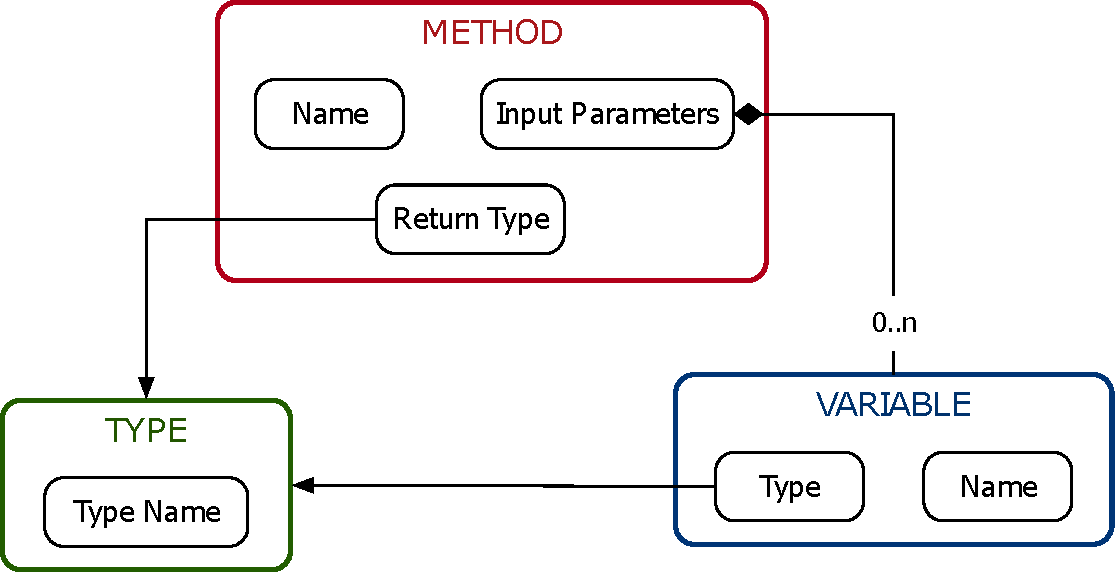
\includegraphics[width=0.8\textwidth]{gfx/russiandoll}
    \caption{TODO}\label{fig:russiandoll}
\end{figure}

Differently from the first code generation step, the model-to-text does not output a single file, but it generates multiple artefacts. For this reason, the process is divided in multiple phases. The first phase is the set up of all the basic elements of the ROS package, with all the folder in place, it can create the launch files. Messages, services and actions are next in the list, when this phase is complete, the process looks for all the nodes and generates them. The last step is executed concurrently with the nodes generations, since it requires to incrementally fill all the configuration and build files.

\paragraph{Package definition} When implementing ROS nodes by hand, the first step is the creation of the containing package. The same process is followed by the code generator. By parsing the AAXML file, it can detect the definition of the AADL package and use it to create the corresponding ROS one. There is an important parallel between ROS and our AADL definition that makes the creation of packages easier; in ROS, a package is the minimal release unit, this means that all dependencies are package-based, this is true also for AADL, where elements can be defined in different packages and included at the beginning using the \texttt{with} keyword. In summary, from the name of the AADL package the code generator derives the name of the ROS package, and from the the \texttt{with} clause it creates all the necessary package-level dependencies.

Most of the package-creation process is the same for all packages. It defines the correct folder structure (see Section~\ref{sec:ros}), and creates the \textit{package.xml} and \textit{CMakeLists.txt} files. These two files are initially created using all the dependencies information derived from the \texttt{with} clause, and they are later updated incrementally depending on the existence of custom messages and the number of custom nodes.

\paragraph{Launch files} The second set of artefacts created by the model-to-text process are the launch files. In order to create a launch file, it is not necessary for the nodes to exist, for each process only the type (\ie, the compile-time name of the node), the package and the instance name are necessary to setup the structure. All this information is available in the AAXML file before generating any source file.

In our model, we defined a relationship between the hierarchical topology defined by AADL systems, and the structure of launch files. Therefore, the code generator parse the AAXML file looking for nested systems, and each one is converted in a launch file. Starting from the deepest child, the launch files are filled with all the necessary nodes, using the AADL instance name as runtime name, the AADL type as reference type, and, if present, the AADL package as the ROS package. To avoid unnecessary clutter in the architecture, only the connected processes are included in the launch files. Of course this is not limited to connections representing topics, but includes any kind of virtual or physical connection that justifies the role of the component in the system.

The following step of the launch file creation is the remapping of topics. In our model we distinguish between two different naming conventions both defined using properties. One is a port property, it is used during the generation of the source code and specifies the default (\ie, written in the source code) name of the topic. The other is a connection property, it is used when creating launch files to define the runtime name of the communication channel.

Last step is the assignment of parameters. If the designer used AADL properties to specify a configuration file, it is converted in YAML and assigned to the correct node in the launch files.
  
\paragraph{Messages} The next phase of the model-to-text process is the generation of messages. Message types are modelled in AADL by a single data component augmented with a property that specifies its internal structure using ASN.1 or JSON Schema. Data types related to messages are not used in the model as instances, but only to specify the type of a communication, hence they only exist in the package definition. This ``out-of-system'' use makes the code generation process simpler.

The package is analysed to detect all the data component; if they are associated with a message description, the file specified in the property is parsed by the specific code generator (\ie, ASN.1 or JSON Schema) to create in the \texttt{msg} folder of the package all the necessary ROS messages files. While creating the message files, the code generator also updates \textit{package.xml} and \textit{CMakeLists.txt} to include all the necessary messages dependencies and the modules to generate and build ROS message files.

\paragraph{Nodes} The last step of the model-to-text process is the generation of the source code of the nodes. The complexity of this step is significantly reduced by our design of the meta-model. We defined a node in AADL as a process that uses threads as subcomponents evoking specific ROS functionalities. In particular, the \textit{main\_thread} characterises a process as a ROS node, this means that during the automatic code generation process the code generator can easily differentiate between ROS nodes and any other process by identifying the \textit{main\_thread} as a subcomponent.

The code generator analyses the package for any process definition including the \textit{main\_thread} as a subcomponent. For each one starts the process of creating all the necessary source files. Most of the basic C++ code is already defined in the engineered node superclass, therefore it is included directly in the automatic generated node. What the code generator needs to do, is to identify all the potential inner functionalities (\ie, publishers, subscribers and timers) of the node, to do so it uses a AADL thread-based approach. Currently the AAXML to ROS/C++ code generator is implemented to identify five different threads corresponding to specific designs:
\begin{itemize}
\item \texttt{ros::publisher.impl}. It correspond to the \textit{source} component behaviour. In our  engineered ROS node, it is implemented by a periodic timer that calls a publisher at the end. Given this design, the code generator has to generate both the timer with its callback and the declaration of the publisher.
\item \texttt{ros::callback.impl}. It represent the \textit{sink} component behaviour. In this case there is no special design, as in any other ROS node, it is a subscriber that trigger a callback. The code generator needs to declare the subscriber, register it to the correct topic, define the callback method and bind it.
\item \texttt{ros::call\_pub.impl}. This thread combines the previous two to evoke a \textit{filter} component behaviour. Since it is a combination of a subscriber that call a publisher in its callback, the code generator needs to define and generate all the previous elements.
\item \texttt{ros::service\_provider.impl}. This thread is used to define a \textit{reactive} component behaviour. The code generator needs to declare a service, advertise correctly and then declare the method used as callback.
\item \texttt{ros::timer.impl}. This last thread does not correspond to any component behaviour, since it is not use for external interactions. However, ROS timers are useful to define the internal behaviour of the node, thus they are one of the potential thread identified by the code generator. Timers are defined similarly to the other elements, and trigger a callback when they expire.
\end{itemize}
If a component contains a thread of an unknown type, the code generation process continues by ignoring it. Often, the designer needs to include threads implementing special interfaces, for example a device driver may use a custom thread to interface with low-level hardware. Since it is impossible to predict all the possible configurations of a node, we decide to use an approach where the designer still has the flexibility of modelling a complete component, while the code generator will only perform a model-to-text transformation for known designs.

The code generator will create multiple files for the same node. All the implementation relative to the functionalities evoked by the threads is in the main source file of the node placed in the \texttt{src} folder of the package. To complete the generation of the main source file, it is necessary to add two more elements: the decoupled functionalities and the parameter initialisation process.

In both our model and in the generated code, we try to push the decoupling between the domain-specific implementation and the middleware-related code. In the model we achieve this by specifying subprograms as subcomponents of threads and then using the \textit{Source\_Text} properties to include the specific implementation of the subprogram. The code generation will retrieve this implementation and call it in the timer or subscriber callbacks as an external function. However, if the property is not specified, or the file referenced by it does not exist, the code generator will automatically create a corresponding header file that the developer can fill at a later stage. The inclusion of any external function or library is propagated by the code generator to the \textit{CMakeLists.txt} file to maintain the package compilation-ready.

The last step of the node generation process is the definition of the internal state. This is done in a separate file that contains the \textit{parameters} and \textit{variables} structures as defined using ANS.1 or JSON Schema. Since they are basic types, parameters are completely defined and initialised using the default values provided, moreover, they are propagated in the main source filed to setup their interface to the parameters server. Variables are declared in their own structure, and initialised if they have a default value and a basic type. However, if they are a complex variables (see Section~\ref{sec:data}), they are only declared and their complex type is included in the header and propagated in the \textit{CMakeLists.txt} file.

\section{A complete example}
Now that we have completely defined how to model a ROS architecture with a combination of AADL and a data modelling language, and we presented our approach to automatic code generation, we can show a complete example, going from the model to the source code. In this section, we will model a basic architecture composed by two nodes interacting to each other, and show the structure of the output package generated by the automatic programming toolchain.

\begin{figure}[t]
\centering
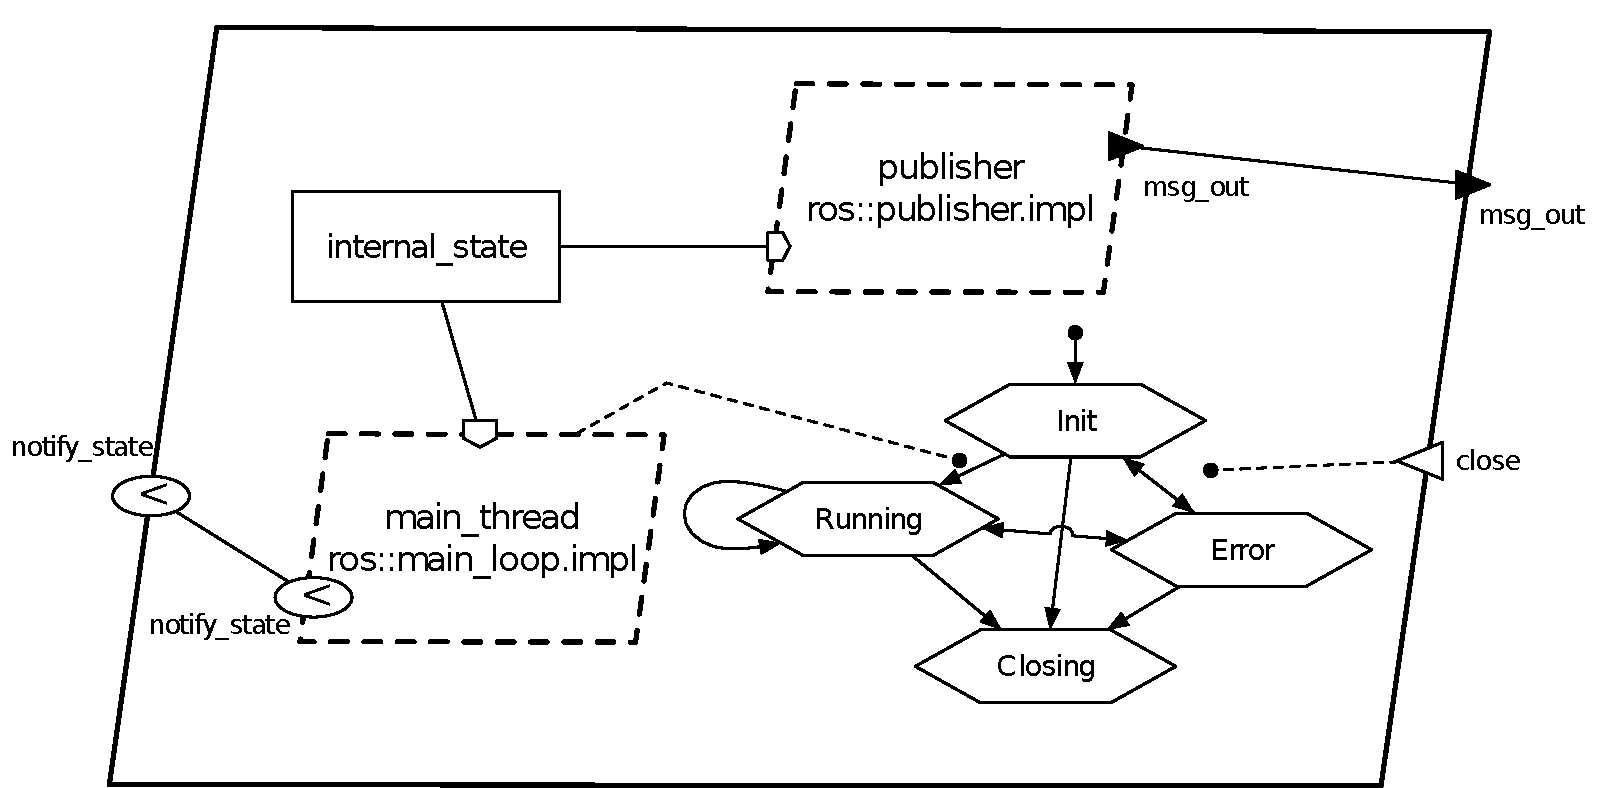
\includegraphics[width=0.95\textwidth]{gfx/usecase-publisher}
\caption{TODO}\label{fig:usecase-publisher}
\end{figure}

The micro architecture in question is the first introductory tutorial provided by the ROS wiki\footnote{http://wiki.ros.org/ROS/Tutorials}, slightly modified to include a custom message: a talker node implementing a publisher and a listener node implementing a subscriber connected through a topic and exchanging messages. Figure~\ref{fig:usecase-publisher} show the graphical representation of the model of the \textit{talker} ROS node. It evokes a \textit{source} component behaviour by generating messages and publishing them on a topic. Additionally to the recurring subcomponents identifying our engineered ROS node (\ie, state machine, main thread and internal state), it models a publisher thread of type \texttt{ros::publisher.impl} communicating with the external environment using a data port specified by the message type. Not visible from the graphical representation are the properties of the node, they are shown in Listing~\ref{lst:tlk-properties}.

\begin{lstlisting}[language=AADL,caption={TODO},label=lst:tlk-properties]
Period => 10 ms applies to publisher;
topic_properties::Default_Name => "/out_chat" applies to msg_out;
Source_Text => ("talker.schema.json") applies to internal_state;
Source_Text => ("talker.h") applies to publisher.function;
Source_Name => "talk" applies to publisher.function;
\end{lstlisting}

\textit{Period} defines the frequency of the publication, the thread will generate a message every 10 ms, this is used by the code generator to define the period of the corresponding ROS timer. \textit{topic\_properties::Default\_Name} represent the name assigned to the topic during implementation when declaring the publisher. There are two \textit{Source\_Text} properties, one for the internal state, to define the structure of parameters and variables, and one points to the header included by the code generator to define the specific functionality of the publisher. This last property is combined with \textit{Source\_Name} to identify the specific function that will output the message to be generated.

\begin{figure}[t]
\centering
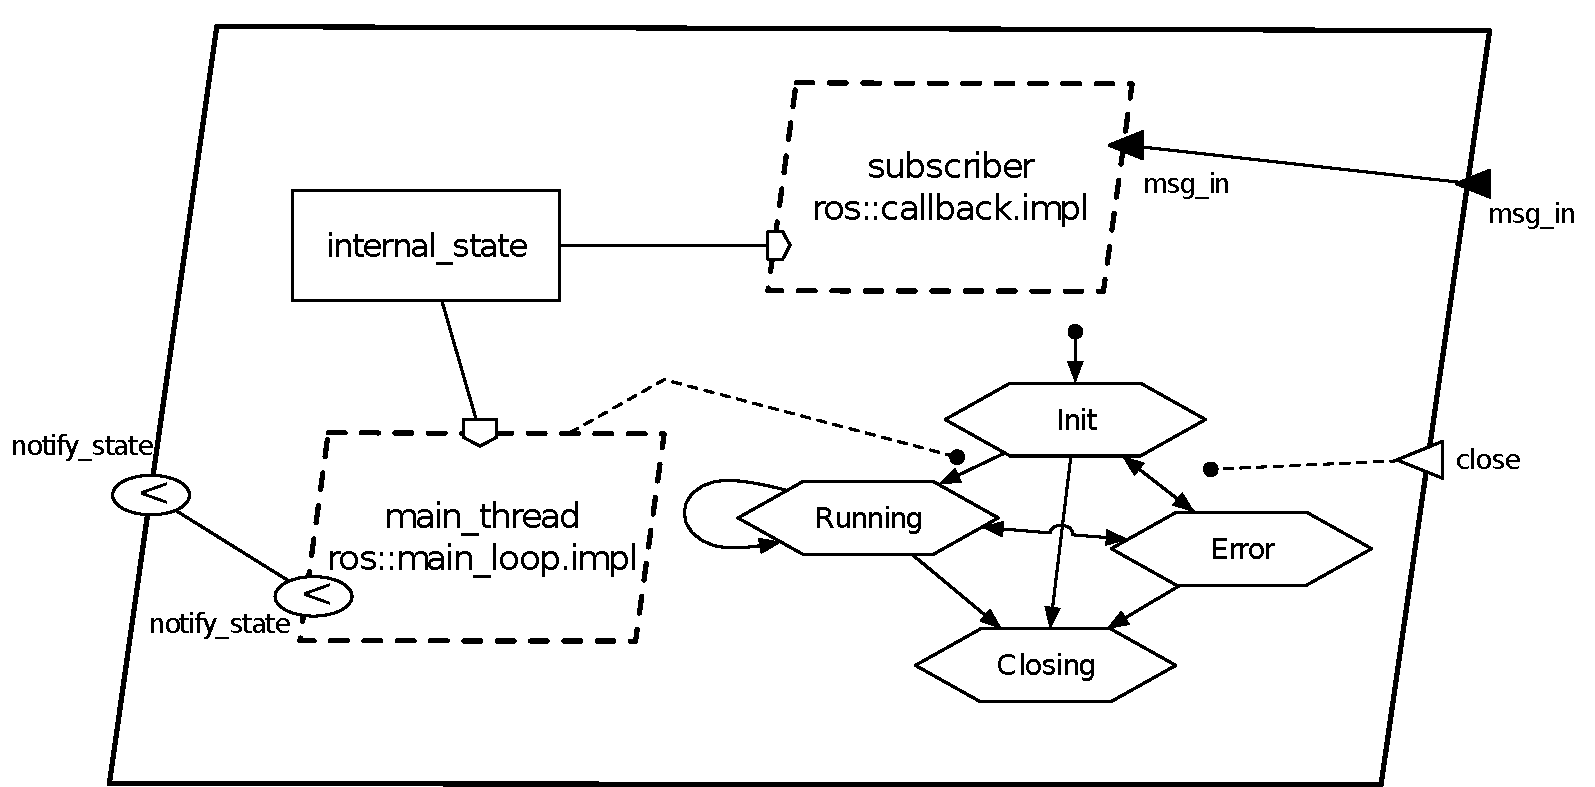
\includegraphics[width=0.95\textwidth]{gfx/usecase-subscriber}
\caption{TODO}\label{fig:usecase-subscriber}
\end{figure}

Figure~\ref{fig:usecase-subscriber} presents the \textit{listener} ROS node graphical AADL model. Since it receives the messages produced by the \textit{talker}, it implements a \textit{sink} component behaviour. As before, the model is composed by the elements characterising the engineered ROS node plus a subscriber thread of type \texttt{ros::callback.impl} receiving data from outside the component through an event data port that triggers the execution of the thread and it is specialised by a specific data component. As for the \textit{talker} node, properties are used to refine the definition of the process, they are detailed in Listing~\ref{lst:lst-properties}

\begin{lstlisting}[language=AADL,caption={TODO},label=lst:lst-properties]
Queue_Size => 1 applies to subscriber.msg;
topic_properties::Default_Name => "/in_chat" applies to msg_in;
Source_Text => ("listener.schema.json") applies to internal_state;
Source_Text => ("listener.h") applies to subscriber.function;
Source_Name => "listen" applies to subscriber.function;
\end{lstlisting}

The properties of \textit{listener} and \textit{talker} are very similar. \textit{Source\_Text} and \textit{Source\_Name} have the same role: defining the internal state of the component and specifying the function to be called during the callback, in this case. Since the subscriber reacts to the messages received, the \textit{Period} property is replaced by \textit{Queue\_Size} that specify the size of the message queue, in this case only the newest message is available. As before, there is a property that defines the name of the topic at compile time, this is the reference name used by the code generator when it creates the definition of the subscriber. It is important to note that the default topic name is different in the two nodes.

Listing~\ref{lst:system} shows the missing element necessary to complete the architecture. At the beginning, the definition of the data component representing the ROS message. The \textit{ChitChat} component is only an interface, its internal structure is defined through a property that points to the JSON schema file used by the code generator to create the ROS message. Follows the implementation of the container, since this is a small architecture with only two components, the root is also the only system. Here the two process instances are declared as subcomponent of the \textit{talking.ros} system, moreover their topic communication is defined using a connection going from the output port of the \textit{talker} to the input port of the \textit{listener}. The properties of the system are used to define the specific runtime configuration of the architecture. \textit{topic\_properties::Name} applied to the connection specifies the remapping of the topic from the original default name used in the implementations. The two \textit{Source\_Text} properties applied directly to the processes are used to define a JSON file that contains a node configuration matching the schema applied in the definition of the components. 

\begin{lstlisting}[language=AADL,caption={TODO},label=lst:system]
data ChitChat
	properties
		Source_Text => ("ChitChat.schema.json");
	end ChitChat;
	
system implementation talking.ros
	subcomponents
		talker: process talker.impl;
		listener: process listener.impl;
	connections
		chatter: port talker.msg_out -> listener.msg_in;
	properties
		topic_properties::Name => "/chatter" applies to chatter;
		Source_Text => ("talker.json") applies to talker;
		Source_Text => ("listener.json") applies to listener;
end talking.ros;
\end{lstlisting}

The AADL model, combined with all the necessary JSON and JSON schema files, is then parsed by the automatic programming toolchain. Since our model included also the source files containing the implementation of the functionalities of the nodes (\ie, \textit{talker.h} and \textit{listener.h}), the output of the process is a complete package ready for compilation. The structure of the package is the following:

\begin{itemize}
	\item[] 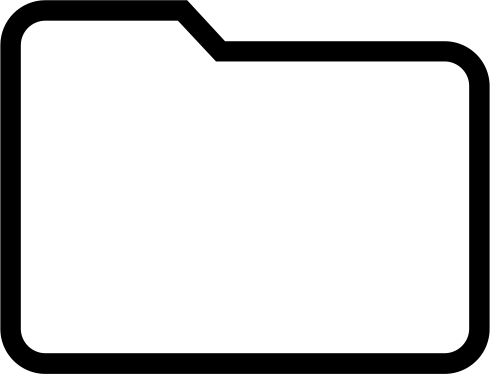
\includegraphics[width=0.3cm]{gfx/tree/folder.png} complete\_example
	\begin{itemize}
	\item[] 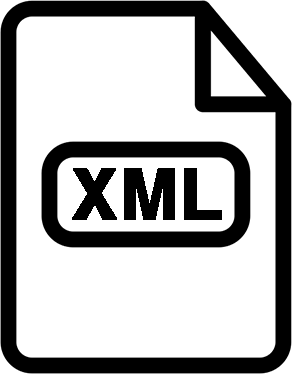
\includegraphics[width=0.3cm]{gfx/tree/file_xml.png} package.xml
	\item[] 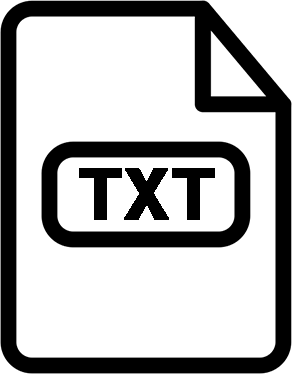
\includegraphics[width=0.3cm]{gfx/tree/file_txt.png} CMakeLists.txt
	\item[] 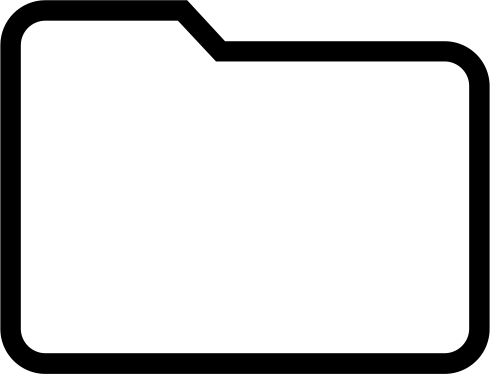
\includegraphics[width=0.3cm]{gfx/tree/folder.png} include
	\begin{itemize}
	\item[] 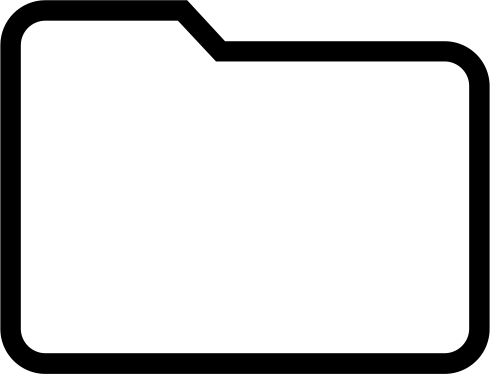
\includegraphics[width=0.3cm]{gfx/tree/folder.png} complete\_example
	\begin{itemize}
	\item[] 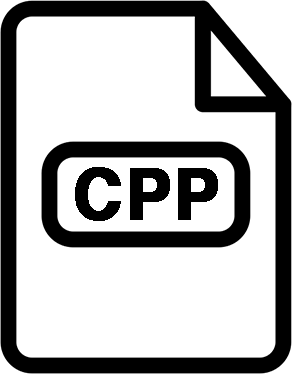
\includegraphics[width=0.3cm]{gfx/tree/file_cpp.png} listener.h
	\item[] 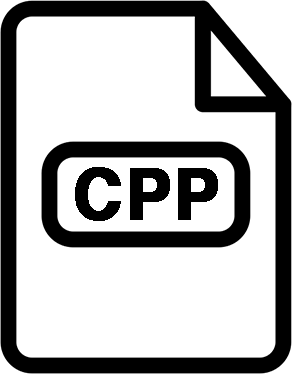
\includegraphics[width=0.3cm]{gfx/tree/file_cpp.png} listener\_configuration.h
	\item[] 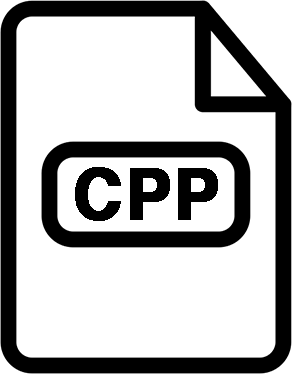
\includegraphics[width=0.3cm]{gfx/tree/file_cpp.png} talker.h
	\item[] 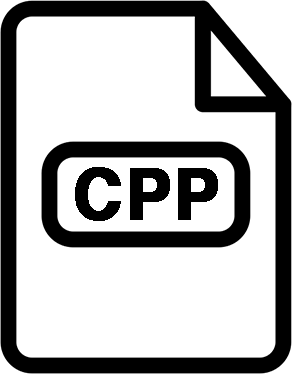
\includegraphics[width=0.3cm]{gfx/tree/file_cpp.png} talker\_configuration.h
	\end{itemize}
	\end{itemize}
	\item[] 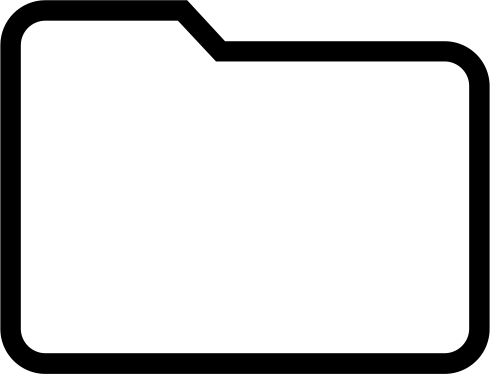
\includegraphics[width=0.3cm]{gfx/tree/folder.png} src
	\begin{itemize}
	\item[] 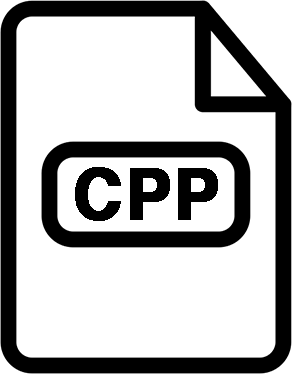
\includegraphics[width=0.3cm]{gfx/tree/file_cpp.png} publisher.cpp
	\item[] 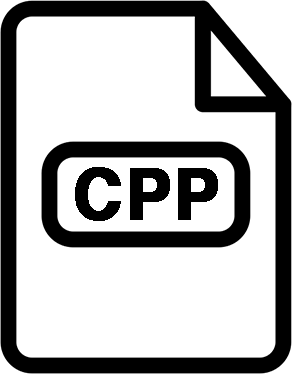
\includegraphics[width=0.3cm]{gfx/tree/file_cpp.png} subscriber.cpp
	\end{itemize}
	\item[] 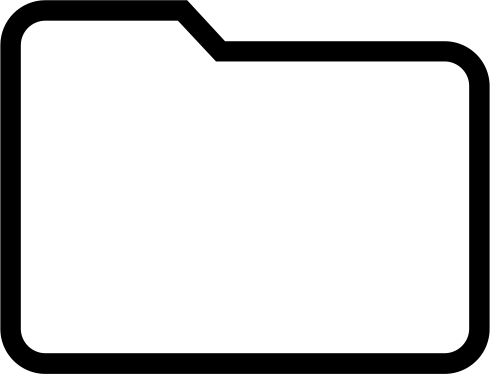
\includegraphics[width=0.3cm]{gfx/tree/folder.png} params
	\begin{itemize}
	\item[] 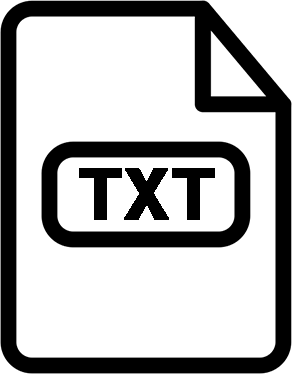
\includegraphics[width=0.3cm]{gfx/tree/file_txt.png} listener.yaml
	\item[] 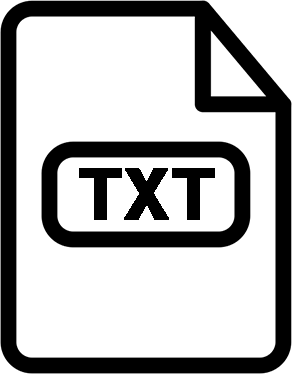
\includegraphics[width=0.3cm]{gfx/tree/file_txt.png} talker.yaml
	\end{itemize}
	\item[] 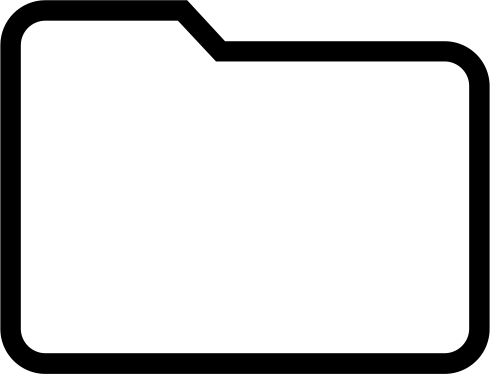
\includegraphics[width=0.3cm]{gfx/tree/folder.png} launch
	\begin{itemize}
	\item[] 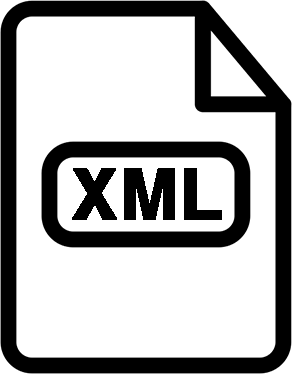
\includegraphics[width=0.3cm]{gfx/tree/file_xml.png} talker.ros.launch
	\end{itemize}
	\item[] 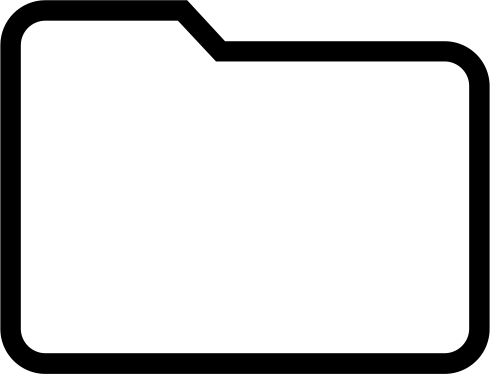
\includegraphics[width=0.3cm]{gfx/tree/folder.png} msg
	\begin{itemize}
	\item[] 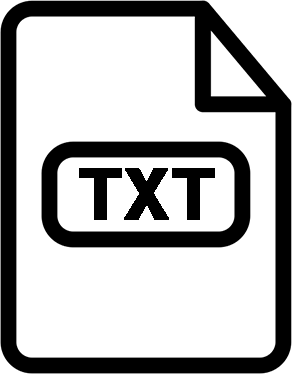
\includegraphics[width=0.3cm]{gfx/tree/file_txt.png} ChitChat.msg
	\end{itemize}
	\end{itemize}
\end{itemize}

%*****************************************
